
    \documentclass{article}
    \usepackage{tikz}
    \usepackage{pgfplots}
    \usepackage{xspace}
    \usetikzlibrary{patterns}
    \newcommand{\capfig}[2]{\textbf{#1}. {\small \textit{#2}}}
    \newcommand{\name}{Verus\xspace}
    \begin{document}

    \begin{figure}
      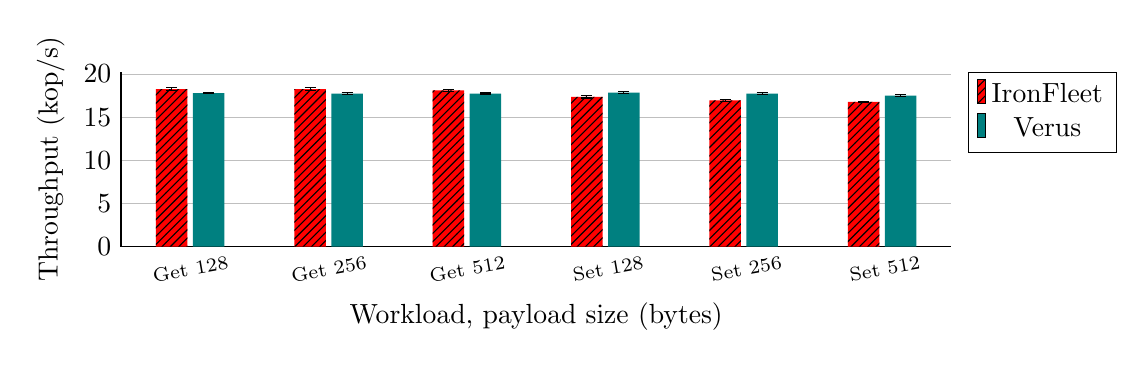
\begin{tikzpicture}
      \centering
      \begin{axis}[
            ybar,
            ymin = 0,
            height=3.8cm, width=\columnwidth,
            legend image code/.code={ \draw [#1] (0cm,-0.1cm) rectangle (0.1cm,0.2cm); },
            legend style={at={(1.2, 1)}},
            bar width=0.4cm,
            ymajorgrids, tick align=inside,
            enlarge y limits={value=.1,upper},
            axis x line*=bottom,
            axis y line*=left,
            x tick label style={rotate=10,anchor=east,xshift=16pt,yshift=-8pt,font=\scriptsize},
            tickwidth=0pt,
            enlarge x limits=true,
            xlabel={Workload, payload size (bytes)},
            ylabel={Throughput (kop/s)},
            symbolic x coords={
               Get 128,Get 256,Get 512,Set 128,Set 256,Set 512
            },
           xtick=data
        ]
    \addplot [draw=none, fill=red!100,postaction={pattern=north east lines},error bars/.cd, y dir=both, y explicit] coordinates {(Get 128,18.247700000000002) += (0, 0.1634290343368079) -= (0, 0.1634290343368079)(Get 256,18.245) += (0, 0.1499049968163675) -= (0, 0.1499049968163675)(Get 512,18.10146) += (0, 0.15285032653435948) -= (0, 0.15285032653435948)(Set 128,17.352203333333332) += (0, 0.13089160423254853) -= (0, 0.13089160423254853)(Set 256,16.940966666666665) += (0, 0.1320751121769348) -= (0, 0.1320751121769348)(Set 512,16.774340000000002) += (0, 0.09023104970930262) -= (0, 0.09023104970930262)};\addplot [draw=none, fill=teal!100,error bars/.cd, y dir=both, y explicit] coordinates {(Get 128,17.793343333333333) += (0, 0.08815154651390245) -= (0, 0.08815154651390245)(Get 256,17.745046666666667) += (0, 0.10737796737405603) -= (0, 0.10737796737405603)(Get 512,17.721529999999998) += (0, 0.08067774232860359) -= (0, 0.08067774232860359)(Set 128,17.84343333333333) += (0, 0.08820105218683238) -= (0, 0.08820105218683238)(Set 256,17.73270333333333) += (0, 0.08807616478019042) -= (0, 0.08807616478019042)(Set 512,17.4909) += (0, 0.10164408457280061) -= (0, 0.10164408457280061)};
        \legend{IronFleet,Verus}
      \end{axis}
      \end{tikzpicture}
       \vspace{-1mm}
      \caption{\capfig{IronKV Performance}
      {
        The \name version performs comparably to the IronFleet original. Each bar shows the mean of 100 trials; error bars show 95\% confidence intervals.\label{fig:ironsht-throughput-comparison}}}
       \vspace{-1mm}
    \end{figure}

    \end{document}
    